%!TEX TS-program = pdflatexmk

% Copyright (c) 2018 - 2022, Martin Scheidt (ISC license)
% Permission to use, copy, modify, and/or distribute this file for any purpose with or without fee is hereby granted, provided that the above copyright notice and this permission notice appear in all copies.

\documentclass[border=2]{standalone}

\usepackage[dev]{tikz-trackschematic}

\begin{document}
  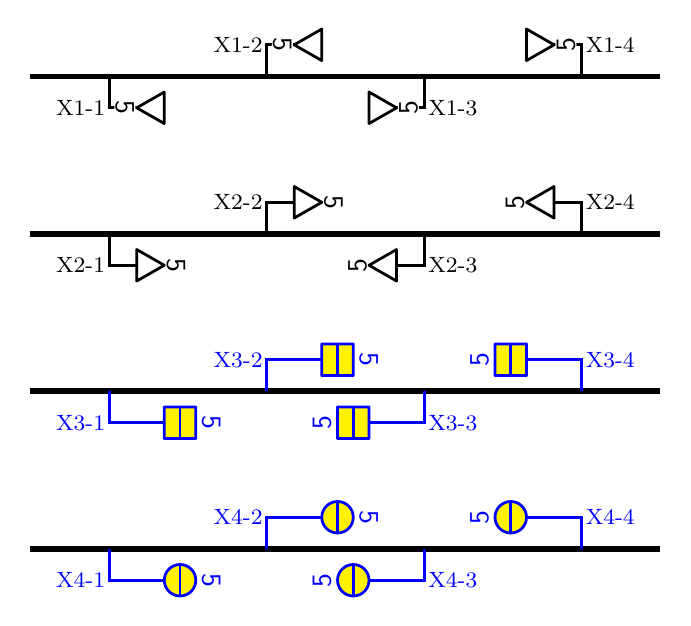
\begin{tikzpicture}

    \foreach \i in {1,2,...,4}{% base coordinate
      \coordinate (A\i) at ($(0,0) + 2*(0,-\i)$);% base coordinate
      \coordinate (B\i) at ($(8,0) + 2*(0,-\i)$);% base coordinate
    }

    \foreach \i in {1,2,...,4}{% draw main tracks on base coordinate
      \maintrack (A\i) --   (B\i);
    }

    \foreach \i in {1,2,...,4}{% coordinates for testing symbols
      \coordinate (X\i-1) at ($(1,0) + 2*(0,-\i)$);
      \coordinate (X\i-2) at ($(3,0) + 2*(0,-\i)$);
      \coordinate (X\i-3) at ($(5,0) + 2*(0,-\i)$);
      \coordinate (X\i-4) at ($(7,0) + 2*(0,-\i)$);
    }


    \colorlet{background}{white}
    \colorlet{foreground}{black}

    \distantsignal[forward ,distant speed=5] at (X1-1) label (X1-1);
    \distantsignal[forward ,distant speed=5,position=left] at (X1-2) label (X1-2);
    \distantsignal[backward,distant speed=5,position=left] at (X1-3) label (X1-3);
    \distantsignal[backward,distant speed=5] at (X1-4) label (X1-4);

    \speedsignal[forward ,speed=5,foreground=blue,background=yellow] at (X2-1) label (X2-1);
    \speedsignal[forward ,speed=5,position=left,foreground=blue,background=yellow] at (X2-2) label (X2-2);
    \speedsignal[backward,speed=5,position=left,foreground=blue,background=yellow] at (X2-3) label (X2-3);
    \speedsignal[backward,speed=5,foreground=blue,background=yellow] at (X2-4) label (X2-4);


    \colorlet{background}{yellow}
    \colorlet{foreground}{blue}

    \blocksignal[forward ,locked,speed=5] at (X3-1) label (X3-1);
    \blocksignal[forward ,locked,speed=5,position=left] at (X3-2) label (X3-2);
    \blocksignal[backward,locked,speed=5,position=left] at (X3-3) label (X3-3);
    \blocksignal[backward,locked,speed=5] at (X3-4) label (X3-4);

    \routesignal[forward ,locked,speed=5,foreground=black,background=white] at (X4-1) label (X4-1);
    \routesignal[forward ,locked,speed=5,position=left,foreground=black,background=white] at (X4-2) label (X4-2);
    \routesignal[backward,locked,speed=5,position=left,foreground=black,background=white] at (X4-3) label (X4-3);
    \routesignal[backward,locked,speed=5,foreground=black,background=white] at (X4-4) label (X4-4);

  \end{tikzpicture}
\end{document}